\section{Introduction}\label{sec:intro}
This lab uses a parallel plate wave guide filled with two different dielectrics to investigate reflection and transmission.
When a uniform plane waves hits the boundary between two different dielectrics part of it is transmitted into the second medium and part of it is reflected back.
The reflected wave interferes with in incident wave and creates a standing wave.
This process is shown in Fig.~\ref{fig:ref_and_trans}.

\begin{figure}[tbph]
	\centering
	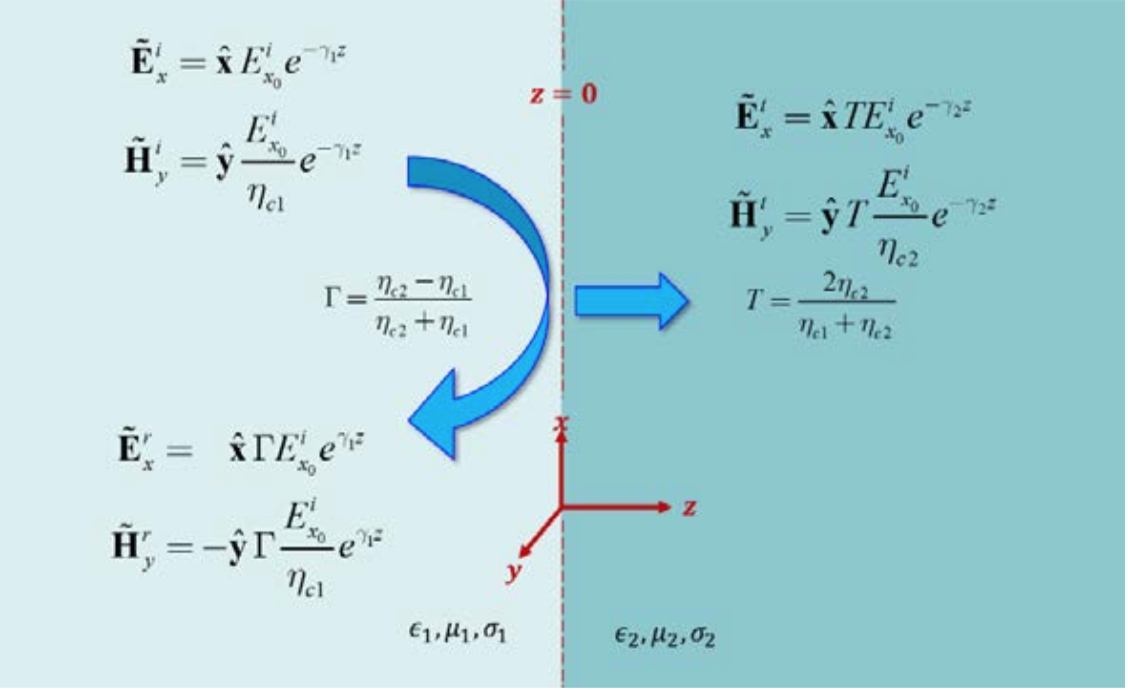
\includegraphics[width=0.7\linewidth]{graphics/ref_and_trans}
	\caption{Reflection and transmission of a uniform plane wave at a normal material boundary}
	\label{fig:ref_and_trans}
\end{figure}

The reflection and transmission coefficientcs, $\Gamma$ and $T$, are given by:
\begin{equation}\label{eqn:coefs}
	\Gamma = { E_{x0}^r \over E_{x0}^i } \qquad\qquad T = { E_{x0}^t \over E_{x0}^i }
\end{equation}

The total electric and magnetic fields in the first material will be the sums of their incident and reflected components.
If the phase of the reflected wave is not \SI{+-90}{\degree}, the total field will have both a traveling and a standing component.
The magnitude of the total wave will be bounded by $E_{x0}^i\left(1 \pm \left|\Gamma\right|\right)$.

For multiple boundaries, this analysis can be applied recursively starting at the medium furthest from the incident wave and working towards it.
